\section{\KLUDGE 概要}

\index{Physics}
Physics\KLUDGE モジュールは物理シミュレーション機能を提供します.
\KLUDGE 主にサポートされているのは,マルチボディダイナミクスと呼ばれる剛体と関節などの拘束からなる動力学シミュレーションです.
\KLUDGE 今のところソフトボディや流体,パーティクルなどの機能はサポートされていません.

\section{Physics SDK}

\index{PHSdk}
Physics\KLUDGE モジュールのすべてのオブジェクトはSDK\KLUDGE クラス\texttt{PHSdk}\KLUDGE によって管理されます.
\texttt{PHSdk}\KLUDGE クラスは,プログラムの実行を通してただ1つのオブジェクトが存在するシングルトンクラスです.
\texttt{PHSdk}\KLUDGE オブジェクトを作成するには以下のようにします.
\begin{sourcecode}
PHSdkIf* phSdk = PHSdkIf::CreateSdk();
\end{sourcecode}
\KLUDGE 通常この操作はプログラムの初期化時に一度だけ実行します.
\KLUDGE また,Framework\KLUDGE モジュールを使用する場合はユーザが直接\texttt{PHSdk}\KLUDGE を作成する必要はありません.

\texttt{PHSdk}\KLUDGE の機能はシーンと形状の管理です.
\KLUDGE シーンに関する機能は次節で説明します.
\KLUDGE また,形状に関する機能は以下の通りです.

\begin{center}
\begin{tabular}{p{.15\hsize}p{.55\hsize}p{.2\hsize}}
\texttt{PHSdkIf} & &															\\ \midrule
\texttt{CDShapeIf*} & \texttt{CreateShape(const CDShapeDesc\&)}	& \KLUDGE 形状を作成	\\
\texttt{CDShapeIf*}	& \texttt{GetShape(int)}					& \KLUDGE 形状を取得	\\
\texttt{int}		& \texttt{NShape()}							& \KLUDGE 形状の数		\\
\end{tabular}
\end{center}

\KLUDGE 異なるシーン間で形状を共有できるように,形状管理はシーンではなく\texttt{PHSdk}\KLUDGE の機能になっています.
\KLUDGE 詳しくは\ref{chap_collision}\KLUDGE 章を参照してください.

\section{\KLUDGE シーン}
\label{sec_physics_scene}

\index{PHScene}
\KLUDGE シーンは物理シミュレーションを行う環境を表します.
\KLUDGE 複数のシーンを作成できますが,シーン同士は互いに独立しており,ユーザが直接橋渡し処理をしない限りは影響を及ぼしあうことはありません.
\KLUDGE シーンクラスは\texttt{PHScene}\KLUDGE で,\texttt{PHScene}\KLUDGE オブジェクトは\texttt{PHSdk}\KLUDGE により管理されます.

\begin{center}
\begin{tabular}{p{.15\hsize}p{.55\hsize}p{.2\hsize}}
\multicolumn{3}{l}{\texttt{PHSdkIf}}															\\ \midrule
\texttt{PHSceneIf*}	& \texttt{CreateScene(const PHSceneDesc\& desc)}			& \KLUDGE シーンを作成		\\
\texttt{int}		& \texttt{NScene()}											& \KLUDGE シーンの数		\\
\texttt{PHSceneIf*}	& \texttt{GetScene(int i)}									& \KLUDGE シーンを取得		\\
\texttt{void}		& \texttt{MergeScene(PHSceneIf* scene0, PHSceneIf* scene1)}	& \KLUDGE シーンを統合		\\
\end{tabular}
\end{center}

\KLUDGE シーンを作成するには以下のようにします.
\begin{sourcecode}
PHSceneIf* phScene = phSdk->CreateScene();
\end{sourcecode}
\KLUDGE 引数にディスクリプタを指定することもできます.
\texttt{MergeScene}\KLUDGE は,\texttt{scene1}\KLUDGE が保有するオブジェクトをすべて\texttt{scene0}\KLUDGE に移動した後に\texttt{scene1}\KLUDGE を削除します.

\KLUDGE シーンは剛体や関節などの様々な構成要素の管理を行うほか,物理シミュレーションに関する設定を行う機能を提供します.
\KLUDGE 各構成要素の作成についてはそれぞれの節で説明しますので,以下ではシミュレーション設定機能について述べます.

\begin{center}
\begin{tabular}{p{.15\hsize}p{.35\hsize}p{.4\hsize}}
\multicolumn{3}{l}{\texttt{PHSceneDesc}}										\\ \midrule
\texttt{double}		&	\texttt{timeStep}	& \KLUDGE 時間ステップ幅					\\
\texttt{unsigned}	&	\texttt{count}		& \KLUDGE シミュレーションしたステップ数	\\
\texttt{Vec3d}		&	\texttt{gravity}	& \KLUDGE 重力加速度						\\
\texttt{double}		&	\texttt{airResistanceRate}	& \KLUDGE 空気抵抗係数				\\
\texttt{int}		&	\texttt{numIteration}		& LCP\KLUDGE の反復回数				\\
\end{tabular}
\end{center}

\begin{center}
\begin{tabular}{p{.15\hsize}p{.55\hsize}p{.2\hsize}}
\multicolumn{3}{l}{\texttt{PHSceneIf}}							  \\ \midrule
\texttt{double}		& \texttt{GetTimeStep()}					& \\
\texttt{void}		& \texttt{SetTimeStep(double)}				& \\
\texttt{unsigned}	& \texttt{GetCount()}						& \\
\texttt{void}		& \texttt{SetCount(unsigned)}				& \\
\texttt{void}		& \texttt{SetGravity(const Vec3d\&)}		& \\
\texttt{Vec3d}		& \texttt{GetGravity()}						& \\
\texttt{void}		& \texttt{SetAirResistanceRate(double)}		& \\
\texttt{double}		& \texttt{GetAirResistanceRate()}			& \\
\texttt{int}		& \texttt{GetNumIteration()}				& \\
\texttt{void}		& \texttt{SetNumIteration()}				& \\
\end{tabular}
\end{center}

\texttt{timeStep}\KLUDGE は一度のシミュレーションステップで進める時間幅です.
\KLUDGE 小さいほどシミュレーションの精度は上がりますが,同じ時間シミュレーションを進めるのにかかる計算コストは増大します.

\texttt{count}\KLUDGE はシーン作成後にシミュレーションした累積ステップ数です.
\texttt{count}\KLUDGE と\texttt{timeStep}\KLUDGE の積が経過時間を表します.

\texttt{gravity}\KLUDGE は重力加速度ベクトルです.

\texttt{airResistanceRate}\KLUDGE は,シミュレーションの安定性を向上するために毎ステップに各剛体の速度に掛けられる係数です.
\KLUDGE 例えば\texttt{airRegistanceRate}\KLUDGE が$0.95$\KLUDGE であればステップごとに速度が$95$\%\KLUDGE になります.
\KLUDGE このように強制的に減速をかけることで,精度を犠牲に安定性を得ることができます.

\texttt{numIteration}\KLUDGE は,拘束力を計算するために内部で実行されるアルゴリズムの反復回数です.
\KLUDGE 一般に,反復回数に関して指数関数的に拘束力の精度が向上し,計算コストは比例的に増大します.

\subsection*{\KLUDGE シミュレーションの実行}

\KLUDGE シミュレーションを$1$\KLUDGE ステップ進めるには\texttt{Step}\KLUDGE 関数を呼びます.

\begin{center}
\begin{tabular}{p{.15\hsize}p{.3\hsize}p{.45\hsize}}
\multicolumn{3}{l}{\texttt{PHSceneIf}}		\\ \midrule
\texttt{void}	& \texttt{Step()}	& \KLUDGE シミュレーションを$1$\KLUDGE ステップ進める \\
\end{tabular}
\end{center}

\texttt{Step}\KLUDGE を実行すると,おおまかに述べて内部で次の処理が行われます.
\begin{itemize}
\item \KLUDGE 衝突判定と接触拘束の生成
\item \KLUDGE 拘束力の計算
\item \KLUDGE 剛体の速度および位置の更新
\end{itemize}

\section{\KLUDGE 剛体}

\index{PHSolid}
\KLUDGE 剛体は物理シミュレーションの基本要素です.
\KLUDGE 剛体のクラスは\texttt{PHSolid}\KLUDGE です.
\KLUDGE まず剛体を作成・管理するための\texttt{PHScene}\KLUDGE の関数を示します.

\begin{center}
\begin{tabular}{p{.15\hsize}p{.45\hsize}p{.30\hsize}}
\multicolumn{3}{l}{\texttt{PHSceneIf}}									\\ \midrule
\texttt{PHSolidIf*}		& \texttt{CreateSolid(const PHSolidDesc\&)}	& \KLUDGE 剛体を作成する \\
\texttt{int}			& \texttt{NSolids()}						& \KLUDGE 剛体の数 \\
\texttt{PHSolidIf**} 	& \texttt{GetSolids()}						& \KLUDGE 剛体配列の先頭アドレス \\
\end{tabular}
\end{center}

\KLUDGE 剛体を作成するには
\begin{sourcecode}
PHSolidIf* solid = phScene->CreateSolid();
\end{sourcecode}
\KLUDGE とします.ディスクリプタを指定して作成することもできます.
\KLUDGE また,\texttt{GetSolids}\KLUDGE は作成した剛体を格納した内部配列の先頭アドレスを返します.
\KLUDGE したがって,例えば$0$\KLUDGE 番目の剛体を取得するには
\begin{sourcecode}
PHSolidIf* solid = phScene->GetSolids()[0];      // get 0-th solid
\end{sourcecode}
\KLUDGE とします.

\KLUDGE つぎに剛体自身の機能を説明します.

\subsection*{\KLUDGE 物性}

\begin{center}
\begin{tabular}{p{.15\hsize}p{.45\hsize}p{.30\hsize}}
\multicolumn{3}{l}{\texttt{PHSolidDesc}}							\\ \midrule
\texttt{double}		&	\texttt{mass}		& \KLUDGE 質量					\\
\texttt{Matrix3d}	&	\texttt{inertia}	& \KLUDGE 慣性行列				\\
\texttt{Vec3d}		&	\texttt{center}		& \KLUDGE 質量中心				\\
\texttt{bool}		&	\texttt{dynamical}	& \KLUDGE 物理法則にしたがうか	\\
\end{tabular}
\end{center}

\begin{center}
\begin{tabular}{p{.15\hsize}p{.45\hsize}p{.30\hsize}}
\multicolumn{3}{l}{\texttt{PHSolidIf}}								\\ \midrule
\texttt{double}		& \texttt{GetMass()}						& \\
\texttt{double} 	& \texttt{GetMassInv()}						& \\
\texttt{void} 		& \texttt{SetMass(double)}					& \\
\texttt{Vec3d} 		& \texttt{GetCenterOfMass()}				& \\
\texttt{void} 		& \texttt{SetCenterOfMass(const Vec3d\&)}	& \\
\texttt{Matrix3d} 	& \texttt{GetInertia()}						& \\
\texttt{Matrix3d} 	& \texttt{GetInertiaInv()}					& \\
\texttt{void} 		& \texttt{SetInertia(const Matrix3d\&)}		& \\
\texttt{void} 		& \texttt{CompInertia()}					& \\
\texttt{void} 		& \texttt{SetDynamical(bool)}				& \\
\texttt{bool} 		& \texttt{IsDynamical()}					& \\
\end{tabular}
\end{center}

\texttt{GetMassInv}\KLUDGE と\texttt{GetInertiaInv}\KLUDGE はそれぞれ質量の逆数と慣性行列の逆行列を返します.
\texttt{CompInertia}\KLUDGE は,その剛体が持つ形状とそれらの密度をもとに剛体の質量,質量中心と慣性行列を計算し,設定します.
\texttt{dynamical}\KLUDGE は,その剛体が物理法則に従うかどうかを指定するフラグです.
\KLUDGE もし\texttt{dynamical}\KLUDGE が\texttt{true}\KLUDGE の場合,その剛体に加わる力が計算され,
\KLUDGE ニュートンの運動法則にしたがって剛体の速度が変化します.
\KLUDGE 一方,\texttt{dynamical}\KLUDGE が\texttt{false}\KLUDGE の場合は外力による影響を受けず,設定された速度で等速運動します.
\KLUDGE これはちょうど∞の質量をもつ場合と同じです.


\subsection*{\KLUDGE 状態}

\begin{center}
\begin{tabular}{p{.15\hsize}p{.45\hsize}p{.30\hsize}}
\multicolumn{3}{l}{\texttt{PHSolidDesc}}							\\ \midrule
\texttt{Vec3d}	&	\texttt{velocity}		& \KLUDGE 速度					\\
\texttt{Vec3d}	&	\texttt{angVelocity}	& \KLUDGE 角速度				\\
\texttt{Posed}	&	\texttt{pose}			& \KLUDGE 位置と向き			\\
\end{tabular}
\end{center}

\begin{center}
\begin{tabular}{p{.2\hsize}p{.5\hsize}p{.20\hsize}}
\multicolumn{3}{l}{\texttt{PHSolidIf}}									\\ \midrule
\texttt{Vec3d}			& \texttt{GetVelocity()}						& \\
\texttt{void} 			& \texttt{SetVelocity(const Vec3d\&)}			& \\
\texttt{Vec3d} 			& \texttt{GetAngularVelocity()}					& \\
\texttt{void} 			& \texttt{SetAngularVelocity(const Vec3d\&)}	& \\
\texttt{Posed} 			& \texttt{GetPose()}							& \\
\texttt{void} 			& \texttt{SetPose(const Posed\&)}				& \\
\texttt{Vec3d} 			& \texttt{GetFramePosition()}					& \\
\texttt{void} 			& \texttt{SetFramePosition(const Vec3d\&)}		& \\
\texttt{Vec3d} 			& \texttt{GetCenterPosition()}					& \\
\texttt{void} 			& \texttt{SetCenterPosition(const Vec3d\&)}		& \\
\texttt{Quaterniond} 	& \texttt{GetOrientation()}						& \\
\texttt{void} 			& \texttt{SetOrientation(const Quaterniond\&)}	& \\
\end{tabular}
\end{center}

\texttt{velocity}, \texttt{angVelocity}, \texttt{pose}\KLUDGE はそれぞれグローバル座標系に関する剛体の速度,角速度,位置および向きを表します.
\texttt{[Get|Set]FramePosition}\KLUDGE はグローバル座標系に関する剛体の位置を取得/\KLUDGE 設定します.
\KLUDGE これに対して\texttt{[Get|Set]CenterPosition}\KLUDGE は剛体の質量中心の位置を取得/\KLUDGE 設定します.
\KLUDGE 偏心している剛体はローカル座標原点と質量中心が一致しないことに注意してください.
\texttt{[Get|Set]Orientation}\KLUDGE はグローバル座標系に関する剛体の向きを取得/\KLUDGE 設定します.


\subsection*{\KLUDGE 力の印加と取得}

\KLUDGE 剛体に加わる力には
\begin{itemize}
\item \KLUDGE ユーザが設定する外力
\item \KLUDGE 重力
\item \KLUDGE 関節や接触から加わる拘束力
\end{itemize}
\KLUDGE の$3$\KLUDGE 種類があり,それぞれについて並進力とトルクがあります.
\KLUDGE ここで,重力は重力加速度と剛体の質量より決まり,拘束力は拘束条件を満たすように内部で自動的に計算されます.
\KLUDGE 以下ではユーザが剛体に加える外力を設定・取得する方法を示します.

\begin{center}
\begin{tabular}{p{.2\hsize}p{.5\hsize}p{.20\hsize}}
\multicolumn{3}{l}{\texttt{PHSolidIf}}								\\ \midrule
\texttt{void} 	& \texttt{AddForce(Vec3d)}					& \\
\texttt{void} 	& \texttt{AddTorque(Vec3d)}					& \\
\texttt{void} 	& \texttt{AddForce(Vec3d, Vec3d)}			& \\
\texttt{Vec3d} 	& \texttt{GetForce()}						& \\
\texttt{Vec3d} 	& \texttt{GetTorque()}						& \\
\end{tabular}
\end{center}

\KLUDGE 並進力を加えるには\texttt{AddForce}\KLUDGE を使います.
\begin{sourcecode}
solid->AddForce(Vec3d(0.0, -1.0, 0.0));
\end{sourcecode}
\KLUDGE とすると剛体の質量中心に並進力$(0, -1, 0)$\KLUDGE が加わります.ただし力はグローバル座標系で表現されます.
\KLUDGE 一方
\begin{sourcecode}
solid->AddTorque(Vec3d(1.0, 0.0, 0.0));
\end{sourcecode}
\KLUDGE とすると剛体の質量中心に関してモーメント$(1, 0, 0)$\KLUDGE が加わります.
\KLUDGE 作用点を任意に指定するには
\begin{sourcecode}
solid->AddForce(Vec3d(0.0, -1.0, 0.0), Vec3d(0.0, 0.0, 1.0));
\end{sourcecode}
\KLUDGE とします.この場合は並進力$(0, -1, 0)$\KLUDGE が作用点$(0, 0, 1)$\KLUDGE に加わります.
\KLUDGE ここで作用点の位置は剛体のローカル座標ではなくグローバル座標で表現されることに注意してください.
\texttt{AddForce}\KLUDGE や\texttt{AddTorque}\KLUDGE は複数回呼ぶと,それぞれで指定した外力の合力が最終的に剛体に加わる外力となります.

\KLUDGE 外力を取得するには\texttt{GetForce}\KLUDGE ,\texttt{GetTorque}\KLUDGE を使います.
\KLUDGE ただし,これらの関数で取得できるのは直前のシミュレーションステップで剛体に作用した外力です.
\KLUDGE したがって直前のシミュレーションステップ後に\texttt{AddForce}\KLUDGE した力は取得できません.
%\KLUDGE シミュレーションの実行と力の印加,取得に関するフローをFig.\,\ref{fig_addforce}\KLUDGE に示します.


\section{\KLUDGE 関節}

\begin{figure}[t]
\begin{center}
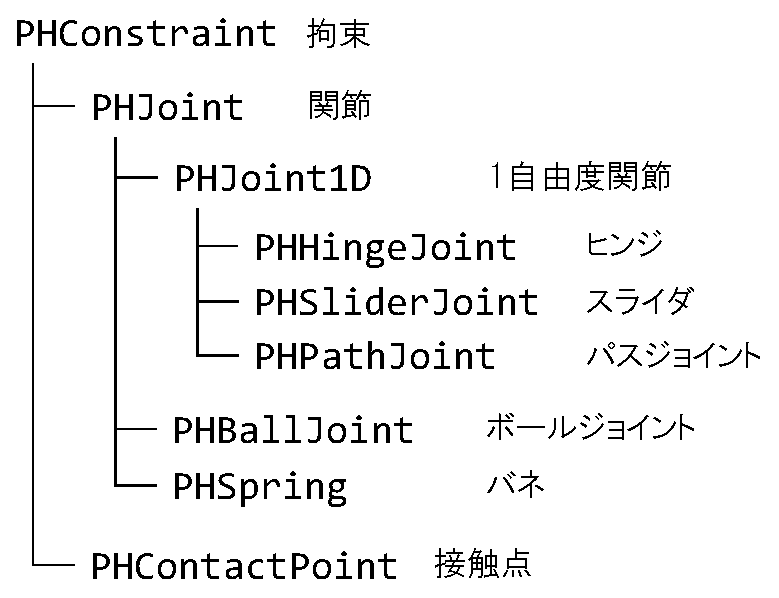
\includegraphics[width=.5\hsize]{fig/phconstraint.eps}
\end{center}
\caption{Constraint class hierarchy}
\label{fig_phconstraint}
\end{figure}

\index{PHConstraint}
\index{PHJoint}
\KLUDGE 拘束とは剛体と剛体の間に作用してその相対的運動に制約を加える要素です.
\KLUDGE 拘束のクラス階層をFig.\,\ref{fig_phconstraint}\KLUDGE に示します.
\KLUDGE まず拘束は関節と接触に分かれます.関節はユーザが作成しますが,接触は衝突判定結果にもとづいて自動的に生成・削除されます.
\KLUDGE 関節はさらにいくつかの種類に分けられます.

\KLUDGE 細かな説明は後回しにして,まずは関節の作成方法から見ていきます.

\subsection*{\KLUDGE 関節の作成}

\KLUDGE 以下ではもっとも使用頻度の高いヒンジの作成を例にとって関節の作成方法を説明します.
\KLUDGE ヒンジを作成するには次のようにします.
\begin{sourcecode}
PHSolidIf* solid0 = phScene->GetSolids()[0];
PHSolidIf* solid1 = phScene->GetSolids()[1];

PHHingeJointDesc desc;
desc.poseSocket.Pos() = Vec3d( 1.0, 0.0, 0.0);
desc.posePlug.Pos()   = Vec3d(-1.0, 0.0, 0.0);
PHHingeJointIf* joint
    = phScene->CreateJoint(solid0, solid1, desc)->Cast();
\end{sourcecode}
\KLUDGE 作成したい関節の種類に応じたディスクリプタを作成し,これを\texttt{PHScene}\KLUDGE の\texttt{CreateJoint}\KLUDGE 関数に渡して関節を作成します.
\KLUDGE このとき,ディスクリプタとともに連結したい剛体のインタフェースも渡します.
\texttt{CreateJoint}\KLUDGE は\texttt{PHJointIf*}\KLUDGE を返しますので,作成した関節のインタフェースを得るには\texttt{Cast}\KLUDGE で動的キャストします.

\KLUDGE 関節に関する\texttt{PHScene}\KLUDGE の関数を以下に示します.

\begin{center}
\begin{tabular}{p{.15\hsize}p{.75\hsize}p{.0\hsize}}
\multicolumn{3}{l}{\texttt{PHSceneIf}}													\\ \midrule
\texttt{PHJointIf*}	& \texttt{CreateJoint(PHSolidIf*, PHSolidIf*, const PHJointDesc\&)}	& \\
\texttt{int}		& \texttt{NJoint()}													& \\
\texttt{PHJointIf*}	& \texttt{GetJoint(int i)}											& \\
\end{tabular}
\end{center}

\texttt{NJoint}\KLUDGE はシーン中の関節の個数を返します.\texttt{GetJoint}\KLUDGE は\texttt{i}\KLUDGE 番目の関節を取得します.


\subsection*{\KLUDGE ソケットとプラグ}

\index{\KLUDGE そけっと@\KLUDGE ソケット}
\index{\KLUDGE ぷらぐ@\KLUDGE プラグ}
\begin{figure}[t]
\begin{center}
\begin{tabular}{c}
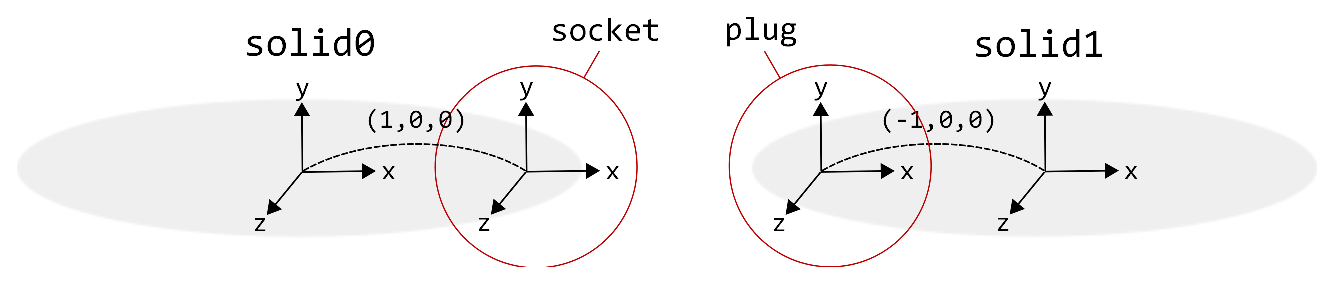
\includegraphics[clip, width=.5\hsize]{fig/socket_plug1.eps} \\
(a) before connection \\
\\
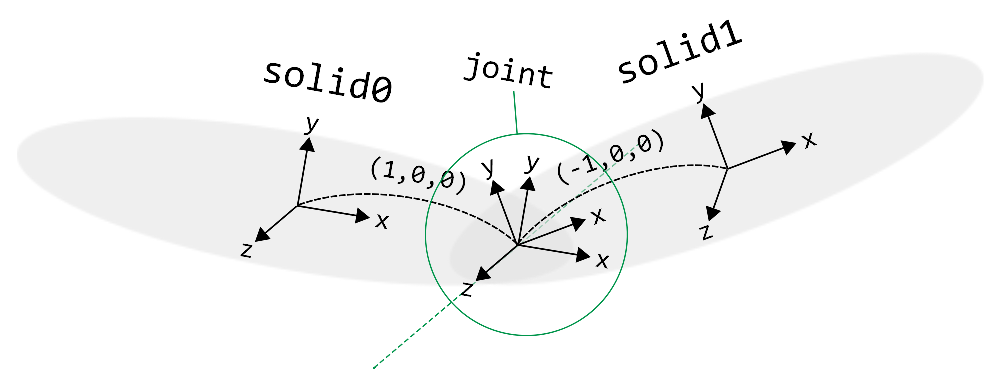
\includegraphics[clip, width=.5\hsize]{fig/socket_plug2.eps} \\
(b) after connection \\
\end{tabular}
\end{center}
\caption{Socket and plug}
\label{fig_socket_plug}
\end{figure}


\KLUDGE さて,上の例でディスクリプタに値を設定している箇所に注目してください.この部分で関節の取り付け位置を指定しています.
Springhead\KLUDGE では,ソケットとプラグと呼ばれるローカル座標系を用いて関節の取り付け位置を表現します.
\KLUDGE ソケットとプラグとは,その名前から連想するように,連結する剛体に取り付ける金具のようなものです.
\texttt{CreateJoint}\KLUDGE の第$1$\KLUDGE 引数の剛体にソケットがつき,第$2$\KLUDGE 引数の剛体にプラグがつきます.
\KLUDGE ソケットとプラグがそれぞれの剛体のどの位置に取り付けられるかを指定するのがディスクリプタの\texttt{poseSocket}\KLUDGE と\texttt{posePlug}\KLUDGE です.
\KLUDGE 上の例ではソケットの位置が$(1,0,0)$\KLUDGE ,プラグの位置が$(-1,0,0)$\KLUDGE でした(Fig.\,\ref{fig_socket_plug}(a))\KLUDGE .
\KLUDGE この場合はFig.\,\ref{fig_socket_plug}(b)\KLUDGE のように剛体が連結されます.
\KLUDGE 後述するように,ヒンジはソケットとプラグのz\KLUDGE 軸を一致させる拘束です.
\KLUDGE したがって連結された剛体同士はソケットとプラグのz\KLUDGE 軸を回転軸として相対的に回転することができます.

\KLUDGE ソケットとプラグに関するディスクリプタとインタフェースを紹介します.

\begin{center}
\begin{tabular}{p{.15\hsize}p{.35\hsize}p{.40\hsize}}
\multicolumn{3}{l}{\texttt{PHConstraintDesc}}					\\ \midrule
\texttt{Posed}	&	\texttt{poseSocket}	& \KLUDGE ソケットの位置と向き	\\
\texttt{Posed}	&	\texttt{posePlug}	& \KLUDGE プラグの位置と向き	\\
\end{tabular}
\end{center}

\begin{center}
\begin{tabular}{p{.15\hsize}p{.50\hsize}p{.25\hsize}}
\multicolumn{3}{l}{\texttt{PHConstraintIf}}								\\ \midrule
\texttt{PHSolidIf*}	& \texttt{GetSocketSolid()}							& \KLUDGE ソケット側の剛体 \\
\texttt{PHSolidIf*} & \texttt{GetPlugSolid()}							& \KLUDGE プラグ側の剛体 \\
\texttt{void} 		& \texttt{GetSocketPose(Posed\&)}					& \\
\texttt{void} 		& \texttt{SetSocketPose(const Posed\&)}				& \\
\texttt{void} 		& \texttt{GetPlugPose(Posed\&)}						& \\
\texttt{void} 		& \texttt{SetPlugPose(const Posed\&)}				& \\
\texttt{void} 		& \texttt{GetRelativePose(Posed\&)}					& \KLUDGE 相対的な位置と向き \\
\texttt{void} 		& \texttt{GetRelativeVelocity(Vec3d\&, Vec3d\&)}	& \KLUDGE 相対速度 \\
\texttt{void} 		& \texttt{GetConstraintForce(Vec3d\&, Vec3d\&)}		& \KLUDGE 拘束力 \\
\end{tabular}
\end{center}
%	Vec3d GetMotorf();
%	Vec3d GetLimitf();

\texttt{GetRelativePose}\KLUDGE はソケット座標系から見たプラグ座標系の相対的な位置と向きを取得します.
\KLUDGE 同様に,\texttt{GetRelativeVelocity}\KLUDGE はソケットからみたプラグの相対速度をソケット座標系で取得します.
\KLUDGE ここで第$1$\KLUDGE 引数が並進速度,第$2$\KLUDGE 引数が角速度です.
\texttt{GetConstraintForce}\KLUDGE はこの拘束が剛体に加えた拘束力を取得します(\KLUDGE 第$1$\KLUDGE 引数が並進力,第$2$\KLUDGE 引数がモーメント)\KLUDGE .
\KLUDGE 具体的には,ソケット側剛体に作用した拘束力をソケット座標系で表現したものが得られます.
\KLUDGE プラグ側剛体には作用反作用の法則によって逆向きの力が作用しますが,これを直接取得する関数は用意されていません.





% --- --- --- --- --- --- --- --- --- --- --- --- --- --- ---
\subsection*{\KLUDGE 関節の種類}

Springhead\KLUDGE で使用可能な関節の種類は

\begin{itemize}
\item \KLUDGE ヒンジ (\texttt{PHHingeIf})
\item \KLUDGE スライダ (\texttt{PHSliderIf})
\item \KLUDGE パスジョイント (\texttt{PHPathJointIf})
\item \KLUDGE ボールジョイント (\texttt{PHBallJointIf})
\item \KLUDGE バネ (\texttt{PHSpringIf})
\end{itemize}

\KLUDGE の5\KLUDGE 種類です.種類ごとに,自由度・拘束の仕方・変位の求め方が異なります.


% --- --- --- --- ---
\subsubsection*{\KLUDGE ヒンジ}

\begin{fig}
\epscapopt{phhingejoint}{Hinge joint}{width=0.5\hsize}
\end{fig}

\index{PHHingeJoint}
\index{\KLUDGE ひんじ@\KLUDGE ヒンジ}
\KLUDGE ヒンジは$1$\KLUDGE 軸回転関節です.
\KLUDGE ヒンジは,\Fig{phhingejoint}\KLUDGE に示すようにソケットとプラグのz\KLUDGE 軸が一致するように拘束します.
\KLUDGE このときソケットのy\KLUDGE 軸とプラグのy\KLUDGE 軸の成す角(x\KLUDGE 軸同士でも同じことですが)\KLUDGE が関節変位となります.

\KLUDGE 関節変位を取得するAPI\KLUDGE は$1$\KLUDGE 自由度関節(\texttt{PH1DJointIf})\KLUDGE で共通です.そのためヒンジに限らずスライダ・パスジョイントでも使用できます.

\begin{reference}{PH1DJointIf}
\classmember{double GetPosition()}
\KLUDGE 関節の変位を取得します.変位のはかり方は関節の種類に依存します.
\end{reference}

% --- --- --- --- ---
\subsubsection*{\KLUDGE スライダ}

\begin{fig}
\epscapopt{phsliderjoint}{Slider joint}{width=0.5\hsize}
\end{fig}

\index{PHSliderJoint}
\index{\KLUDGE すらいだ@\KLUDGE スライダ}
\KLUDGE スライダは$1$\KLUDGE 自由度の直動関節です.
\KLUDGE スライダは,\Fig{phsliderjoint}\KLUDGE に示すようにソケットとプラグのz\KLUDGE 軸が同一直線上に乗り,かつ両者のx\KLUDGE 軸,y\KLUDGE 軸が同じ向きを向くように拘束します.
\KLUDGE このときソケットの原点からプラグの原点までが関節変位となります.



% --- --- --- --- ---
\subsubsection*{\KLUDGE パスジョイント}

\index{PHPathJoint}
\index{\KLUDGE ぱすじょいんと@\KLUDGE パスジョイント}
\KLUDGE パスジョイントはソケットとプラグの相対位置関係を$1$\KLUDGE パラメータの自由曲線で表現する関節です.詳しくは後述します.

T.B.D.



% --- --- --- --- ---
\subsubsection*{\KLUDGE ボールジョイント}

\begin{fig}
  \begin{tabular}{cc}
    \epsopt{phballjoint}{width=0.45\hsize} & \epsopt{swingtwist}{width=0.35\hsize} \\
    (a) & (b)
  \end{tabular}
  \labelcap{phballjoint}{Ball Joint}
\end{fig}

\index{PHBallJoint}
\index{\KLUDGE ぼーるじょいんと@\KLUDGE ボールジョイント}
\KLUDGE ボールジョイントは$3$\KLUDGE 自由度の回転関節です.
\KLUDGE ボールジョイントは\Fig{phballjoint}(a)\KLUDGE に示すようにソケットとプラグの原点が一致するように拘束します.
\KLUDGE ソケット座標系をプラグ座標系に変換するようなクォータニオンが変位となります.

\KLUDGE 一方で,ボールジョイントの変位はオイラー角の一種であるSwing-Twist\KLUDGE 座標系(\Fig{phballjoint}(b))\KLUDGE で取得することもできます.
\KLUDGE ソケットとプラグのz\KLUDGE 軸同士がなす角をスイング角(Swing)\KLUDGE ,プラグのz\KLUDGE 軸をソケットのx-y\KLUDGE 平面への射影がソケットのx\KLUDGE 軸となす角をスイング方位角(Swing-Dir)\KLUDGE ,プラグのz\KLUDGE 軸周りの回転角度をツイスト角(Twist)\KLUDGE と呼びます.Swing-Twist\KLUDGE 座標系は,後述するボールジョイントの関節可動範囲の指定に用います.

\KLUDGE この2\KLUDGE 種類の変位は,それぞれに対応した関数で取得することができます.
\begin{reference}{PHBallJoint}
\classmember{Quaterniond GetPosition()}
\KLUDGE ソケット座標系をプラグ座標系に変換するようなクォータニオンを返します.

\classmember{Vec3d GetAngle()}
Swing-Twist\KLUDGE 座標系で表現された関節変位を返します.
\end{reference}


\subsubsection*{\KLUDGE バネ}

\index{PHSpring}
\index{\KLUDGE ばね@\KLUDGE バネ}

\begin{fig}
\epscapopt{phspring}{Spring}{width=0.5\hsize}
\end{fig}

\KLUDGE 剛体間を連結するダンパ付きバネです.ソケット座標系とプラグ座標系が一致するときが自然状態で,位置の変位・姿勢の変位に比例して自然状態に戻すような力・モーメントを発生します.並進運動に作用するバネ・ダンパ係数と,回転運動に作用するバネ・ダンパ係数はディスクリプタによってそれぞれ設定できます.

\begin{lightreference}{PHSpringDesc}
% \member\KLUDGE マクロがうまく機能しない
%\member{Vec3d spring}{\KLUDGE 並進運動に対するバネ係数}
%\member{Vec3d damper}{\KLUDGE 並進運動に対するダンパ係数}
%\member{double springOri}{\KLUDGE 回転運動に対するバネ係数}
%\member{double damperOri}{\KLUDGE 回転運動に対するダンパ係数}
\multicolumn{2}{l}{\texttt{Vec3d spring}} & \KLUDGE 並進運動に対するバネ係数 \\
\multicolumn{2}{l}{\texttt{Vec3d damper}} & \KLUDGE 並進運動に対するダンパ係数 \\
\multicolumn{2}{l}{\texttt{double springOri}} & \KLUDGE 回転運動に対するバネ係数 \\
\multicolumn{2}{l}{\texttt{double damperOri}} & \KLUDGE 回転運動に対するダンパ係数 \\
\end{lightreference}


\subsection*{\KLUDGE 有効化と無効化}

\begin{center}
\begin{tabular}{p{.15\hsize}p{.45\hsize}p{.30\hsize}}
\multicolumn{3}{l}{\texttt{PHConstraintDesc}}					\\ \midrule
\texttt{bool}	&	\texttt{bEnabled}	& \KLUDGE 有効/\KLUDGE 無効フラグ		\\
\end{tabular}
\end{center}

\begin{center}
\begin{tabular}{p{.15\hsize}p{.50\hsize}p{.25\hsize}}
\multicolumn{3}{l}{\texttt{PHConstraintIf}}						\\ \midrule
\texttt{void}	& \texttt{Enable(bool)}					& \\
\texttt{bool} 	& \texttt{IsEnabled()}					& \\
\end{tabular}
\end{center}

\KLUDGE 有効な拘束は拘束力を生じます.無効化された拘束は存在しないのと同じ状態になりますが,
\KLUDGE 削除するのと異なりいつでも再度有効化することができます.
\KLUDGE 作成直後の拘束は有効化されています.





\subsection*{\KLUDGE 関節制御}

\subsubsection*{$1$\KLUDGE 自由度関節の場合}

\begin{center}
\begin{tabular}{p{.15\hsize}p{.45\hsize}p{.30\hsize}}
\multicolumn{3}{l}{\texttt{PHJoint1DDesc}}								\\ \midrule
\texttt{double}	&	\texttt{spring}			& \KLUDGE 可動範囲下限				\\
\texttt{double}	&	\texttt{damper}			& \KLUDGE 可動範囲上限				\\
\texttt{double}	&	\texttt{targetPosition}	& \KLUDGE 可動範囲制限用バネ係数	\\
\texttt{double}	&	\texttt{targetVelocity}	& \KLUDGE 可動範囲制限用ダンパ係数	\\
\texttt{double}	&	\texttt{offsetForce}	& \\
\texttt{double}	&	\texttt{fMax}			& \\
\end{tabular}
\end{center}

\begin{center}
\begin{longtable}{p{.15\hsize}p{.45\hsize}p{.30\hsize}}
\multicolumn{3}{l}{\texttt{PHJoint1DIf}}						\\ \midrule
\texttt{double}	& \texttt{GetPosition()}				& \KLUDGE 関節変位を取得 \\
\texttt{double} & \texttt{GetVelocity()}				& \KLUDGE 関節速度を取得 \\
\texttt{void} 	& \texttt{SetSpring(double)}			& \\
\texttt{double} & \texttt{GetSpring()}					& \\
\texttt{void} 	& \texttt{SetDamper(double)}			& \\
\texttt{double} & \texttt{GetDamper()}					& \\
\texttt{void} 	& \texttt{SetTargetPosition(double)}	& \\
\texttt{double} & \texttt{GetTargetPosition()}			& \\
\texttt{void} 	& \texttt{SetTargetVelocity(double)}	& \\
\texttt{double} & \texttt{GetTargetVelocity()}			& \\
\texttt{void} 	& \texttt{SetOffsetForce(double)}		& \\
\texttt{double} & \texttt{GetOffsetForce()}				& \\
\texttt{void} 	& \texttt{SetTorqueMax(double)}			& \KLUDGE 最大関節トルクを設定 \\
\texttt{double} & \texttt{GetTorqueMax()}				& \KLUDGE 最大関節トルクを取得 \\
\end{longtable}
\end{center}

\KLUDGE 関節を駆動する力$f$\KLUDGE は次式で与えられます.
\begin{align*}
f = K(p_0 - p) + D(v_0 - v) + f_0
\end{align*}
\KLUDGE ここで$p$\KLUDGE ,$v$\KLUDGE はそれぞれ関節変位と関節速度で\texttt{GetPosition}\KLUDGE ,\texttt{GetVelocity}\KLUDGE で取得できます.
\KLUDGE その他の記号とディスクリプタ変数との対応は以下の通りです.
\begin{center}
\begin{tabular}{ll}
$K$		&	\texttt{spring}				\\
$D$		&	\texttt{damper}				\\
$p_0$	&	\texttt{targetPosition}		\\
$v_0$	&	\texttt{targetVelocity}		\\
$f_0$	&	\texttt{offsetForce}
\end{tabular}
\end{center}
\KLUDGE 上の式はバネ・ダンパモデルとPD\KLUDGE 制御則の二通りの解釈ができます.
\KLUDGE 前者としてとらえるなら$K$\KLUDGE はバネ係数,$D$\KLUDGE はダンパ係数,$p_0$\KLUDGE はバネの自然長,$v_0$\KLUDGE は基準速度となります.
\KLUDGE 後者としてとらえる場合は$K$\KLUDGE はP\KLUDGE ゲイン,$D$\KLUDGE はD\KLUDGE ゲイン,$p_0$\KLUDGE は目標変位,$v_0$\KLUDGE は目標速度となります.
\KLUDGE また,$f_0$\KLUDGE は関節トルクのオフセット項です.
\KLUDGE 上の式で得られた関節トルクは最後に$\pm$\texttt{fMax}\KLUDGE の範囲に収まるようにクランプされます.

\subsubsection*{\KLUDGE ボールジョイントの場合}

\KLUDGE ヒンジと同様に,バネダンパモデル・PD\KLUDGE 制御を実現します.
\KLUDGE ボールジョイントの変位はクォータニオンで表されるため,目標変位\texttt{targetPosition}\KLUDGE はクォータニオンで,目標速度\texttt{targetVelocity}\KLUDGE は回転ベクトルで与えます.

\begin{lightreference}{PHBallJointDesc}
% \member\KLUDGE マクロがうまく機能しない
%\member{double spring}{\KLUDGE バネ係数}
%\member{double damper}{\KLUDGE ダンパ係数}
%\member{Quaterniond targetPosition}{\KLUDGE 目標変位}
%\member{Vec3d targetVelocity}{\KLUDGE 目標速度}
%\member{Vec3d offsetForce}{\KLUDGE モータートルク}
%\member{double fMax}{\KLUDGE 関節トルクの限度}
\multicolumn{2}{l}{\texttt{double spring}} & \KLUDGE バネ係数 \\
\multicolumn{2}{l}{\texttt{double damper}} & \KLUDGE ダンパ係数 \\
\multicolumn{2}{l}{\texttt{Quaterniond targetPosition}} & \KLUDGE 目標変位 \\
\multicolumn{2}{l}{\texttt{Vec3d targetVelocity}} & \KLUDGE 目標速度 \\
\multicolumn{2}{l}{\texttt{Vec3d offsetForce}} & \KLUDGE モータートルク \\
\multicolumn{2}{l}{\texttt{double fMax}} & \KLUDGE 関節トルクの限度 \\
\end{lightreference}



	%\multicolumn{2}{l}{\texttt{void SetMotorTorque(double)}}		& \\
	%\multicolumn{2}{l}{\texttt{double GetMotorTorque()}}	& \\

	%double	secondDamper;	///< \KLUDGE 二個目のダンパ係数
	%double  yieldStress;	///< \KLUDGE 降伏応力
	%double  hardnessRate;	///< \KLUDGE 降伏応力以下の場合に二個目のダンパ係数に掛ける比率

	%void SetTrajectoryVelocity(double v);
	%double GetTrajectoryVelocity();
	%double  GetSecondDamper();
	%void	SetSecondDamper(double input);
	%double GetYieldStress();
    %void SetYieldStress(const double yS);
	%double GetHardnessRate();
	%void SetHardnessRate(const double hR);
	%PHJointDesc::PHDeformationType 	GetDeformationMode();





% --- --- --- --- --- --- --- --- --- --- --- --- --- --- ---
\subsection*{\KLUDGE 可動域制限}

\texttt{CreateLimit}\KLUDGE は可動範囲制約オブジェクトのディスクリプタを引数にとります.
$1$\KLUDGE 自由度関節の可動範囲制約の場合,\texttt{Vec2d range}\KLUDGE が可動域を表します.\texttt{range[0]}\KLUDGE が可動域の下限,\texttt{range[1]}\KLUDGE が上限です.\texttt{range[0] < range[1]}\KLUDGE が満たされているときに限り可動範囲制約が有効となります.
\KLUDGE デフォルトでは\texttt{range[0] > range[1]}\KLUDGE となる値が設定されていて,可動範囲制約は無効となっています.

\KLUDGE 関節の変位が可動範囲限界に到達したとき,範囲を超過しないように可動範囲制約の拘束力が作用します.
\KLUDGE このとき,関節変位を範囲内に押し戻す力はバネ・ダンパモデルで計算されます.
\KLUDGE このバネ係数とダンパ係数はそれぞれディスクリプタの\texttt{spring}\KLUDGE ,\texttt{damper}\KLUDGE で指定します.

\begin{tips}
\KLUDGE 可動範囲用の\texttt{spring}\KLUDGE ,\texttt{damper}\KLUDGE は初期値でも十分大きな値が設定されていますが,関節制御において非常に大きなバネ・ダンパ係数を用いると可動範囲制約のバネ・ダンパが負けてしまうことがあります.その場合には関節制御より大きな係数を適切に再設定すると,可動範囲内で関節を制御する事ができるようになります.
\end{tips}


\subsubsection*{$1$\KLUDGE 自由度関節の場合}

\begin{reference}{PH1DJointLimitDesc}
\classmember{Vec2d range}
\KLUDGE 可動範囲を表します.\texttt{range[0]}\KLUDGE が下限,\texttt{range[1]}\KLUDGE が上限です.

\classmember{double spring} \Plus
\classmember{double damper}
\KLUDGE 可動範囲を制限するためのバネ・ダンパモデルの係数です.
\end{reference}

\begin{reference}{PH1DJointLimitIf}
\classmember{IsOnLimit()}
\KLUDGE 現在の関節姿勢が可動範囲外にある時に\texttt{true}\KLUDGE を返します.この関数が\texttt{true}\KLUDGE を返すような時,関節には可動域制約を実現するための拘束力が発生しています.
\end{reference}


\subsubsection*{\KLUDGE ボールジョイントの場合}

\KLUDGE ボールジョイントの可動範囲は\Fig{phballjoint}(b)\KLUDGE に示すSwing-Twist\KLUDGE 座標系によって指定します.

\KLUDGE ボールジョイントに対しては2\KLUDGE 種類の可動範囲制約を使用することができます.
\begin{itemize}
\item \texttt{ConeLimit}\KLUDGE は円錐形の可動範囲制約で,主に関節のスイング角を一定範囲内に制約します.
\item \texttt{SplineLimit}\KLUDGE は自由曲線形の可動範囲制約で,プラグ座標系z\KLUDGE 軸の可動範囲を閉曲線で指定することができます.
\end{itemize}

\KLUDGE ここでは\texttt{ConeLimit}\KLUDGE について説明します(\texttt{SplineLimit}\KLUDGE については後述します)\KLUDGE .

\begin{reference}{PHBallJointConeLimitDesc}
\classmember{Vec2d limitSwing}
\KLUDGE スイング角の可動範囲です.概念的には,関節が一定以上に折れ曲がらないようにする制約です(\KLUDGE スイング角の下限を設定する事もできるので,実際には一定以上にまっすぐにならないようにする機能も有しています)\KLUDGE .

\texttt{limitSwing[0]}\KLUDGE が下限,\texttt{limitSwing[1]}\KLUDGE が上限です.\texttt{limitSwing}\KLUDGE を取得・設定するためのAPI\KLUDGE は
\begin{quote}
\texttt{PHBallJointConeLimitIf::[Set|Get]SwingRange(range)}
\end{quote}
\KLUDGE です.

\texttt{limitSwing[0] > limitSwing[1]}\KLUDGE となる時は無効化されます.デフォルトでは\texttt{limitSwing[0] > limitSwing[1]}\KLUDGE となる値がセットされています.

\classmember{Vec2d limitTwist}
\KLUDGE ツイスト角の可動範囲です.概念的には,関節が一定以上にねじれないようにするための制約です.

\texttt{limitTwist[0]}\KLUDGE が下限,\texttt{limitTwist[1]}\KLUDGE が上限です.\texttt{limitTwist}\KLUDGE を取得・設定するためのAPI\KLUDGE は
\begin{quote}
\texttt{PHBallJointConeLimitIf::[Set|Get]TwistRange(range)}
\end{quote}
\KLUDGE です.

\texttt{limitTwist[0] > limitTwist[1]}\KLUDGE となる時は無効化されます.デフォルトでは\texttt{limitTwist[0] > limitTwist[1]}\KLUDGE となる値がセットされています.

\classmember{double spring} \Plus
\classmember{double damper}
\KLUDGE 可動範囲を制限するためのバネ・ダンパモデルの係数です.$1$\KLUDGE 自由度関節の場合と同じです.
\end{reference}

\begin{reference}{PHBallJointConeLimitIf}
\classmember{IsOnLimit()}
\KLUDGE 現在の関節姿勢が可動範囲外にある時に\texttt{true}\KLUDGE を返します.$1$\KLUDGE 自由度関節の場合と同じです.
\end{reference}



% --- --- --- --- --- --- --- --- --- --- --- --- --- --- ---
\subsection*{\KLUDGE ボールジョイントの自由曲線可動域} \label{sec_splinelimit}





% --- --- --- --- --- --- --- --- --- --- --- --- --- --- ---
\subsection*{\KLUDGE パスジョイント} \label{sec_phpathjoint}



% --- --- --- --- --- --- --- --- --- --- --- --- --- --- ---
\subsection*{\KLUDGE 弾塑性変形バネダンパ}







\section{\KLUDGE 関節系の逆運動学}

% ----- ----- ----- ----- ----- ----- ----- ----- ----- ----- ----- ----- ----- ----- ----- ----- ----- -----
%
% \KLUDGE 概説
% 

\KLUDGE 逆運動学(IK)\KLUDGE は,剛体関節系において剛体が目標位置に到達するよう関節を制御する機能です.

Springhead\KLUDGE では,関節系のヤコビアンを用いたIK\KLUDGE 機能が使用可能です.
\KLUDGE 物理シミュレーションの1\KLUDGE ステップごとに関節系のヤコビアンを計算し,それに基づいて剛体を目標位置・姿勢に近づけるような各関節の角速度を計算します.
\KLUDGE シミュレーションを続けることで,最終的に剛体が目標位置・姿勢となった状態が得られます.

Springhead\KLUDGE 上の剛体関節系に対してIK\KLUDGE を使用するには,少々下準備が必要です.
\KLUDGE 次のように3\KLUDGE つの剛体が直線状につながった関節系を例にとって解説します.

\begin{center}
\epsopt{ikexample3link}{width=0.5\hsize}
\end{center}


% ----- ----- ----- ----- ----- ----- ----- ----- ----- ----- ----- ----- ----- ----- ----- ----- ----- -----
%
% \KLUDGE 例
% 

IK\KLUDGE を使用するには,まずIK\KLUDGE に用いるための関節を「アクチュエータ」として登録する必要があります.
\begin{sourcecode}
// given PHSceneIf* phScene
// given PHSolidIf* solid1, solid2, solid3
// given PHHingeJointIf* joint1 (solid1 <-> solid2)
// given PHHingeJointIf* joint2 (solid2 <-> solid3)

PHIKHingeActuatorDesc descIKActuator;

PHIKHingeActuatorIf* ikActuator1
  = phScene->CreateIKActuator(descIKActuator);
ikActuator1.AddChildObject(joint1);

PHIKHingeActuatorIf* ikActuator2
  = phScene->CreateIKActuator(descIKActuator);
ikActuator1.AddChildObject(joint2);
\end{sourcecode}
\texttt{PHIKHingeActuatorIf}\KLUDGE は\texttt{PHHingeJointIf}\KLUDGE に対応するアクチュエータクラスです.


\KLUDGE 次に,関節系の親子関係を登録します.親アクチュエータに,子アクチュエータを登録します.
\begin{sourcecode}
ikActuator1.AddChildObject(ikActuator2);
\end{sourcecode}


\KLUDGE また,IK\KLUDGE を用いて到達させる先端の剛体を「エンドエフェクタ」として登録する必要があります.
\begin{sourcecode}
PHIKEndEffectorDesc descEndEffector;

PHIKEndEffectorIf* ikEndEffector1
  = phScene->CreateIKEndEffector(descEndEffector);
ikEndEffector1.AddChildObject(solid3);
\end{sourcecode}


\KLUDGE 最後に,剛体関節系の親子関係において,エンドエフェクタの直接の親にあたるアクチュエータに対し,エンドエフェクタを登録します.
\begin{sourcecode}
ikActuator2.AddChildObject(ikEndEffector1);
\end{sourcecode}
\KLUDGE この例では \texttt{solid1 -(joint1)-> solid2 -(joint2)-> solid3} \KLUDGE のように関節が接続されていますから,関節系の末端である \texttt{solid3} \KLUDGE をエンドエフェクタにした場合,直接の親にあたるアクチュエータは \texttt{joint2} \KLUDGE に対応するアクチュエータ,すなわち \texttt{ikActuator2} \KLUDGE ということになります.

\KLUDGE ここまでの作業で,生成されたオブジェクトの関係は以下のようになっているはずです.
\begin{center}
\epsopt{ikexample3linkobjects}{width=0.9\hsize}
\end{center}
\KLUDGE これで下準備は終わりです.

\KLUDGE 目標位置をセットし,IK\KLUDGE エンジンを有効にするとIK\KLUDGE が動き始めます.
\begin{sourcecode}
// solid3 goes to (2, 5, 0)
ikEndEffector1->SetTargetPosition(Vec3d(2, 5, 0)); 

phScene->GetIKEngine()->Enable(true);

...
phScene->Step(); // IK is calculated in physics step
...
\end{sourcecode}

% ----- ----- ----- ----- ----- ----- ----- ----- ----- ----- ----- ----- ----- ----- ----- ----- ----- -----
%
% \KLUDGE 詳細
% 

% ----- ----- ----- ----- ----- ----- ----- ----- ----- ----- ----- ----- ----- ----- ----- ----- 
\subsection*{IK\KLUDGE エンジン}
% \KLUDGE 概説

IK\KLUDGE の計算は,\texttt{PHScene}\KLUDGE が持つIK\KLUDGE エンジン(\texttt{PHIKEngine})\KLUDGE によって実現されています.

IK\KLUDGE エンジンはデフォルトでは無効となっています.
\begin{sourcecode}
phScene->GetIKEngine()->Enable(true);
\end{sourcecode}
\KLUDGE を実行することで有効となります.\texttt{GetIKEngine()}\KLUDGE は,\texttt{PHScene}\KLUDGE が持つIK\KLUDGE エンジンを取得するAPI\KLUDGE です.

Springhead\KLUDGE におけるIK\KLUDGE の計算原理は,関節系のヤコビ行列(ヤコビアン)に基づきます.全アクチュエータの関節角度に微小変化量 $\varDelta\bm{\theta}$ \KLUDGE を与えた時の,全エンドエフェクタの位置の微小変化量 $\varDelta\bm{r}$ \KLUDGE は,関節系のヤコビアン $J$ \KLUDGE を用いて
\[
\varDelta\bm{r} = J \varDelta\bm{\theta}
\]
\KLUDGE と表されます.毎ステップごとに関節系ヤコビアン$J$\KLUDGE および目標位置に向かう微小変位$\varDelta\bm{r}$\KLUDGE を計算し,上記の線形連立方程式を解くことで各関節に与える角速度を求めます.

\KLUDGE 線形連立方程式の求解にはガウス=\KLUDGE ザイデル法による繰り返し解法を用いています.そのため1\KLUDGE ステップあたりの繰り返し計算の回数によって計算速度と計算精度のトレードオフがあります.繰り返しの回数は,
\begin{sourcecode}
// 20 iteration per 1 physics step
phScene->GetIKEngine()->SetNumIter(20);
\end{sourcecode}
\KLUDGE のようにして設定することができます.

% ----- ----- ----- ----- ----- ----- ----- ----- ----- ----- ----- ----- ----- 
% \KLUDGE リファレンス
\referencetitle

\begin{reference}{PHSceneIf}
\classmember{PHIKEngineIf* GetIKEngine()}
IK\KLUDGE エンジンを取得します.
\end{reference}

\begin{reference}{PHIKEngineIf}
\classmember{Enable(bool b)}
IK\KLUDGE エンジンの有効・無効を切り替えます.引数が\texttt{true}\KLUDGE ならば有効化し,\texttt{false}\KLUDGE ならば無効化します.

\classmember{SetNumIter(int n)}
IK\KLUDGE の繰り返し計算回数を1\KLUDGE ステップあたり\texttt{n}\KLUDGE 回にセットします.
\end{reference}



% ----- ----- ----- ----- ----- ----- ----- ----- ----- ----- ----- ----- ----- ----- ----- ----- 
\subsection*{\KLUDGE アクチュエータ}
% \KLUDGE 概説

Springhead\KLUDGE では,IK\KLUDGE に使用する各関節をアクチュエータと呼びます.IK\KLUDGE は,アクチュエータを駆動させて剛体を目標位置に到達させます.

\KLUDGE <オブジェクト関係図>

IK\KLUDGE エンジンはアクチュエータを複数保持し,各アクチュエータが各関節を保持します.アクチュエータオブジェクト一つにつき,関節が一つ対応します.
\KLUDGE アクチュエータオブジェクトの具体的な役割は,関節の状態をIK\KLUDGE エンジンに伝え,IK\KLUDGE の計算のうち関節ヤコビアンの計算など関節ごとに行う部分を実行し,IK\KLUDGE の計算結果に従って関節を動かす事です.


% ----- ----- ----- ----- ----- ----- ----- ----- ----- ----- ----- ----- ----- 
% \KLUDGE 詳細
\subsubsection*{\KLUDGE アクチュエータクラスの種類と作成}

\KLUDGE 本稿執筆時点では,IK\KLUDGE 用アクチュエータとして使用できるのはヒンジとボールジョイントのみです.
\KLUDGE それぞれに対応したアクチュエータクラスがあります.

\begin{itemize}
\item \texttt{PHIKHingeActuator}\KLUDGE は\texttt{PHHingeJoint}\KLUDGE に対するアクチュエータです.ヒンジジョイントの1\KLUDGE 自由度を駆動に用います.

\item \texttt{PHIKBallActuator}\KLUDGE は\texttt{PHBallJoint}\KLUDGE に対するアクチュエータです.ボールジョイントは3\KLUDGE 自由度の関節ですが,後述するエンドエフェクタの姿勢制御を行わない(\KLUDGE エンドエフェクタの位置のみを制御する)\KLUDGE 場合は,エンドエフェクタの位置を変化させることのできる2\KLUDGE 自由度のみを駆動に用います(\KLUDGE 使用する2\KLUDGE 自由度の軸は1\KLUDGE ステップごとに更新されます)\KLUDGE .
\end{itemize}

\begin{sourcecode}
// given PHSceneIf* phScene

PHIKHingeActuatorDesc descIKActuator;
PHIKHingeActuatorIf* ikActuator
    = phScene->CreateIKActuator(descActuator);
\end{sourcecode}
\KLUDGE アクチュエータを作成するには,\texttt{PHSceneIf}\KLUDGE の\texttt{CreateIKActuator}\KLUDGE 関数を用います.引数はアクチュエータのディスクリプタです.\texttt{PHIKHingeActuatorDesc}\KLUDGE 型のディスクリプタを渡すとヒンジ用のアクチュエータが作成され,\texttt{PHIKBallActuatorDesc}\KLUDGE 型のディスクリプタを渡すとボールジョイント用のアクチュエータが作成されます.

\KLUDGE 作成された時点では,アクチュエータは関節と対応付けがされていません.アクチュエータの子要素に関節を登録することで対応付けが行われます.
\begin{sourcecode}
// given PHHingeJointIf* joint
ikActuator->AddChildObject(joint);
\end{sourcecode}


% ----- ----- ----- ----- ----- ----- ----- ----- ----- ----- ----- ----- ----- 
% \KLUDGE 詳細
\subsubsection*{\KLUDGE アクチュエータの親子関係の登録}

\KLUDGE 次のように二股に分岐したリンクを例にとります:

\begin{center}
\epsopt{ikexample5link}{width=0.8\hsize}
\end{center}

\KLUDGE 計算上,IK\KLUDGE で駆動する関節系は木構造でなければなりません.
Springhead\KLUDGE では,アクチュエータの親子関係を作ることで関節の木構造を設定します.

\begin{sourcecode}
// given PHIKActuator ikActuator1, ikActuator2
ikActuator1->AddChildObject(ikActuator2);
\end{sourcecode}
\texttt{AddChildObject}\KLUDGE を呼び出すと,アクチュエータに対し「子要素」となるアクチュエータを登録することができます.
\KLUDGE これを全てのアクチュエータに対して行うことでアクチュエータの木構造が設定されます.このときアクチュエータの親子関係は,前出の図の右側のようになります.


% ----- ----- ----- ----- ----- ----- ----- ----- ----- ----- ----- ----- ----- 
% \KLUDGE 詳細
\subsubsection*{\KLUDGE 関節のダンパ係数とIK}

%%% \KLUDGE 位置モード付けるかもしれません.本リリースまでに決めること. %%%

\KLUDGE 関節の運動は,IK\KLUDGE 機能によって計算された目標関節角速度を関節に\texttt{SetTargetVelocity}\KLUDGE することで実現します.
\KLUDGE 目標速度に関する関節の振る舞いは,関節の\texttt{damper}\KLUDGE パラメータによって変化します.一般に\texttt{damper}\KLUDGE が大きいほど関節は固くなり,外乱の影響を受けづらくなります.この性質はそのままIK\KLUDGE の振る舞いにも受け継がれます.


% ----- ----- ----- ----- ----- ----- ----- ----- ----- ----- ----- ----- ----- 
% \KLUDGE 詳細
\subsubsection*{\KLUDGE 重み付きIK}

\KLUDGE 通常,IK\KLUDGE は全ての関節を可能な限り均等に使用して目標を達成するよう計算されます.
\KLUDGE 一方,キャラクタの動作に用いる場合などで,手先を優先的に動かし胴体はあまり動かさない,といった重み付けが要求される場面があります.

Springhead\KLUDGE のIK\KLUDGE には,このような重み付けを設定することができます.
\begin{sourcecode}
// given PHIKActuator ikActuator1, ikActuator2
ikActuator1->SetBias(2.0);
ikActuator2->SetBias(1.0);
\end{sourcecode}
\texttt{SetBias}\KLUDGE は,指定した関節をあまり動かさないように設定する関数です.Bias\KLUDGE には$1.0$\KLUDGE 以上の値を設定します.大きな値を設定した関節ほど,IK\KLUDGE による動作は小さくなります.デフォルトではどのアクチュエータも$1.0$\KLUDGE となっており,全関節が均等に使用されます.

% ----- ----- ----- ----- ----- ----- ----- ----- ----- ----- ----- ----- ----- 
% \KLUDGE リファレンス(アクチュエータ)





% ----- ----- ----- ----- ----- ----- ----- ----- ----- ----- ----- ----- ----- ----- ----- ----- 
\subsection*{\KLUDGE エンドエフェクタ}
% \KLUDGE 概説

\KLUDGE 剛体・関節系を構成する剛体の一部を,「エンドエフェクタ」に指定することができます.
\KLUDGE エンドエフェクタには目標位置・姿勢を指示することができます.IK\KLUDGE エンジンは,エンドエフェクタ剛体が指定された目標位置・姿勢を達成するようアクチュエータを制御します.


% ----- ----- ----- ----- ----- ----- ----- ----- ----- ----- ----- ----- ----- 
% \KLUDGE 詳細
\subsubsection*{\KLUDGE エンドエフェクタの作成}

\KLUDGE エンドエフェクタは\texttt{PHSceneIf}\KLUDGE の\texttt{CreateIKEndEffector}\KLUDGE を用いて作成します.引数には\texttt{PHIKEndEffectorDesc}\KLUDGE を渡します.
\begin{sourcecode}
// given PHSceneIf* phScene

PHIKEndEffectorDesc descEndEffector;

PHIKEndEffectorIf* ikEndEffector
  = phScene->CreateIKEndEffector(descEndEffector);
\end{sourcecode}

\KLUDGE アクチュエータ同様,エンドエフェクタも作成時点では剛体との対応を持ちません.\texttt{AddChildObject}\KLUDGE により剛体を子要素として登録する必要があります.
\begin{sourcecode}
// given PHSolidIf* solid

ikEndEffector.AddChildObject(solid);
\end{sourcecode}

\KLUDGE 次に,エンドエフェクタ剛体を親剛体に連結しているアクチュエータに対し,エンドエフェクタを子要素として登録します.
\begin{sourcecode}
// given PHIKActuatorIf* ikActuatorParent

ikActuatorParent.AddChildObject(ikEndEffector);
\end{sourcecode}
\KLUDGE こうすることでエンドエフェクタはアクチュエータ木構造の葉ノードとなり,IK\KLUDGE の計算に使用できるようになります.

\KLUDGE なお,エンドエフェクタは一つの関節系に対して複数作成することができます.この場合,IK\KLUDGE は複数のエンドエフェクタが可能な限り同時に目標位置・姿勢を達成できるようアクチュエータを制御します.また,エンドエフェクタは関節系の先端剛体に限りません.


% ----- ----- ----- ----- ----- ----- ----- ----- ----- ----- ----- ----- ----- 
% \KLUDGE 詳細
\subsubsection*{\KLUDGE 目標位置の設定}

\KLUDGE エンドエフェクタの目標位置は\texttt{SetTargetPosition}\KLUDGE によって指定します.
\begin{sourcecode}
// solid3 goes to (2, 5, 0)
ikEndEffector->SetTargetPosition(Vec3d(2, 5, 0)); 
\end{sourcecode}

\KLUDGE エンドエフェクタに目標姿勢を指示し,エンドエフェクタが特定の姿勢をとるように関節系を動作させることもできます.
\begin{sourcecode}
ikEndEffector->SetTargetOrientation( Quaterniond::Rot('x', rad(30)) ); 
ikEndEffector->EnableOrientationControl(true);
\end{sourcecode}
\KLUDGE 目標姿勢は\texttt{Quaterniond}\KLUDGE で設定します.姿勢制御はデフォルトでは無効になっており,使用するには\texttt{EnableOrientationControl}\KLUDGE を呼んで有効化する必要があります.

\texttt{EnablePositionControl}\KLUDGE および\texttt{EnableOrientationControl}\KLUDGE を用いると,位置制御・姿勢制御の両方を個別に有効・無効化することができます.
\begin{sourcecode}
// 位置制御あり,姿勢制御なし(デフォルト)
ikEndEffector->EnablePositionControl(true);
ikEndEffector->EnableOrientationControl(false);
\end{sourcecode}

\begin{sourcecode}
// 位置制御なし,姿勢制御あり
ikEndEffector->EnablePositionControl(false);
ikEndEffector->EnableOrientationControl(true);
\end{sourcecode}

\begin{sourcecode}
// 位置制御あり,姿勢制御あり
ikEndEffector->EnablePositionControl(true);
ikEndEffector->EnableOrientationControl(true);
\end{sourcecode}


% ----- ----- ----- ----- ----- ----- ----- ----- ----- ----- ----- ----- ----- 
% \KLUDGE リファレンス(エンドエフェクタ)

\section{\KLUDGE 接触}
\label{sec_physics_contact}

\index{\KLUDGE せっしょく@\KLUDGE 接触}

\subsection*{\KLUDGE 接触モデル}

\begin{figure}[t]
\begin{center}
\begin{tabular}{c}
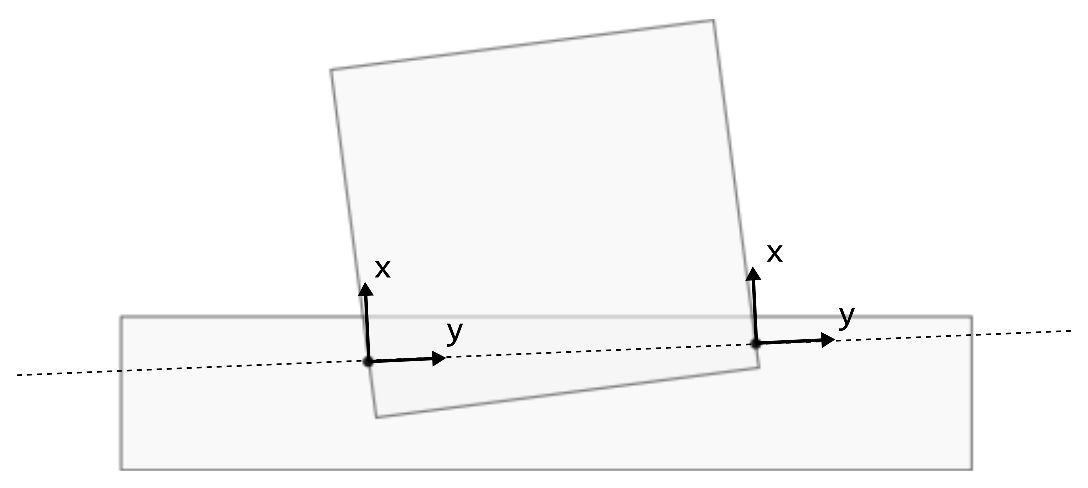
\includegraphics[clip, width=.7\hsize]{fig/phcontact.eps} \\
\end{tabular}
\end{center}
\caption{Contact configuration}
\label{fig_physics_contact}
\end{figure}

Springhead\KLUDGE で採用している接触モデルについて説明します.
\KLUDGE 第\ref{sec_physics_scene}\KLUDGE 節で述べたように,\texttt{PHSceneIf::Step}\KLUDGE によってシミュレーションを1\KLUDGE ステップ進めると,
\KLUDGE 初めに形状の交差判定と接触拘束の生成が行われます.
\KLUDGE 交差する二つの形状の交差断面と,接触拘束の関係についてFig.\,\ref{fig_physics_contact}\KLUDGE に示します.
\KLUDGE 図では簡単のために二次元で描いていますが,実際には接触断面を表す多角形の各頂点に接触拘束が作られます.
\KLUDGE 接触拘束も他の拘束と同様にソケットとプラグで構成されます.
\KLUDGE 一方で,他の拘束とは違い接触拘束は交差判定アルゴリズムによって動的に生成・破棄されます.
\KLUDGE このため,接触し合う剛体のどちらにソケットあるいはプラグが取り付けられるかは状況依存であり,外部から選択することはできません.

\KLUDGE プラグおよびソケットの向きは次のようにして決まります.
\KLUDGE まず,x\KLUDGE 軸は接触法線と平行に向きます.ただしどちらが正の向きかは状況依存です.
\KLUDGE 次に,y\KLUDGE 軸は接触点における二つの剛体の相対速度ベクトルを接触断面へ投影した向きに向きます.
\KLUDGE 最後にz\KLUDGE 軸はx\KLUDGE ,y\KLUDGE 軸に直交するように決まります.

\KLUDGE 以下では各接触拘束が課す条件について具体的に述べます.
\KLUDGE まず,法線方向の進入速度の大小に応じて衝突モデルと静的接触モデルのいずれかが選択されます.
\begin{align*}
v^\mathrm{x} < -V^\mathrm{th}   \;\; &\Rightarrow \;\; \text{\KLUDGE 衝突モデル} \\
v^\mathrm{x} \ge -V^\mathrm{th} \;\; &\Rightarrow \;\; \text{\KLUDGE 静的接触モデル}
\end{align*}
\KLUDGE ここで$v^\mathrm{x}$\KLUDGE はソケットから見たプラグの相対速度のx\KLUDGE 軸(接触法線)成分で,近づき合う向きを負とします.
\KLUDGE また,$V^\mathrm{th}$\KLUDGE は衝突モデルへ切り替わる臨界速度です.

\KLUDGE 衝突モデルでは,1\KLUDGE ステップ後の相対速度${v^\mathrm{x}}'$\KLUDGE が跳ね返り係数$e$\KLUDGE にもとづいて決まり,それを満たすような接触力が計算されます.
\begin{align}
{v^\mathrm{x}}' = - e \, v^\mathrm{x}
\end{align}
\KLUDGE ここで,跳ね返り係数は衝突する形状の物性値に定義された跳ね返り係数の平均値です.
%\KLUDGE 各形状の跳ね返り係数は,\texttt{CDShapeDesc::e}\KLUDGE か,\texttt{CDShapeIf::SetElasticity}\KLUDGE を用いて設定します
%\KLUDGE (第\ref{sec_collision_material}\KLUDGE 節参照).

\KLUDGE 静的接触モデルでは,形状同士の進入深度$d$\KLUDGE が1\KLUDGE ステップで所定の割合で減少するような接触力を求めます.
\KLUDGE つまり,1\KLUDGE ステップ後の進入深度を$d'$\KLUDGE とすると
\begin{align}
d' = d - \gamma \mathrm{max}(d - d^\mathrm{tol}, 0)
\end{align}
\KLUDGE となります.
\KLUDGE ここで$\gamma$\KLUDGE は接触拘束の誤差修正率です.
\KLUDGE また,$d^\mathrm{tol}$\KLUDGE は許容進入深度です.

\KLUDGE 最後に,接触力が満たすべき条件について述べます.
\KLUDGE まず,法線方向には反発力のみ作用することから,接触力のx\KLUDGE 軸成分$f^\mathrm{x}$\KLUDGE には
\begin{align*}
f^\mathrm{x} \ge 0
\end{align*}
\KLUDGE が課せられます.
\KLUDGE 一方で接触力のy\KLUDGE 軸成分$f^\mathrm{y}$\KLUDGE ,z\KLUDGE 軸成分$f^\mathrm{z}$\KLUDGE は摩擦力を表します.
\KLUDGE 摩擦力に関しては,その向きの相対速度にもとづき静止摩擦か動摩擦かが判定され,それに応じて最大摩擦力の制約が課されます.
\begin{align*}
-\mu_0 f^\mathrm{x} \le &f^\mathrm{y} \le \mu_0 f^\mathrm{x} & & \text{if} \; -V^\mathrm{f} \le v^\mathrm{y} \le V^\mathrm{f},\\
 \mu   f^\mathrm{x} \le &f^\mathrm{y} \le \mu   f^\mathrm{x} & & \text{otherwise}
\end{align*}
\KLUDGE ここで,静止摩擦係数$\mu_0$\KLUDGE および動摩擦係数$\mu$\KLUDGE は跳ね返り係数と同様に各形状の物性値の平均値が用いられます.
\KLUDGE また,$V^\mathrm{f}$\KLUDGE は静止摩擦と動摩擦が切り替わる臨界速度です.
z\KLUDGE 軸方向についても同様の制約が課されます.

\KLUDGE 接触モデルの関係するインタフェースには以下があります.
\begin{center}
\begin{longtable}{p{.1\hsize}p{.5\hsize}p{.4\hsize}}
\multicolumn{3}{l}{\texttt{CDShapeIf}}						\\ \midrule
\texttt{void}	& \texttt{SetElasticity(float e)}       & \KLUDGE 跳ね返り係数を設定 \\
\texttt{float}  & \texttt{GetElasticity()}              & \KLUDGE 跳ね返り係数を取得 \\
\texttt{void}   & \texttt{SetStaticFriction(float mu0)} & \KLUDGE 静摩擦係数を設定 \\
\texttt{float}  & \texttt{GetStaticFriction()}          & \KLUDGE 静摩擦係数を取得 \\
\texttt{void}   & \texttt{SetDynamicFriction(float mu)} & \KLUDGE 動摩擦係数を設定 \\
\texttt{float}  & \texttt{GetDynamicFriction()}         & \KLUDGE 動摩擦係数を取得
\end{longtable}
\end{center}

\begin{center}
\begin{longtable}{p{.1\hsize}p{.5\hsize}p{.4\hsize}}
\multicolumn{3}{l}{\texttt{PHSceneIf}}						\\ \midrule
\texttt{void}	& \texttt{SetContactTolerance(double tol)} & \KLUDGE 許容交差深度を設定 \\
\texttt{double} & \texttt{GetContactTolerance()}           & \KLUDGE 許容交差深度を取得 \\
\texttt{void}   & \texttt{SetImpactThreshold(double vth)}  & \KLUDGE 最小衝突速度を設定 \\
\texttt{double} & \texttt{GetImpactThreshold()}            & \KLUDGE 最小衝突速度を取得 \\
\texttt{void}   & \texttt{SetFrictionThreshold(double vf)} & \KLUDGE 最小動摩擦速度を設定 \\
\texttt{double} & \texttt{GetFrictionThreshold()}          & \KLUDGE 最小動摩擦速度を取得
\end{longtable}
\end{center}

\noindent\textbf{\KLUDGE 備考}
\begin{itemize}
\item \KLUDGE 接触断面の向きについては,形状同士の進入速度をもとに決定しますが,ここでは詳しく述べません.
\item \KLUDGE 摩擦力に関してはy\KLUDGE 軸,z\KLUDGE 軸が個別に扱われますが,実際の摩擦力はy\KLUDGE 成分とz\KLUDGE 成分の合力として与えられますので,
\KLUDGE 合力が最大摩擦力を超過する可能性があります.このようにSpringhead\KLUDGE の摩擦モデルはあくまで近似的なものですので
\KLUDGE 注意して下さい.
\end{itemize}

\subsection*{\KLUDGE 接触力の取得}

\KLUDGE 特定の剛体に作用する接触力を直接取得するためのインタフェースは用意されていません.
\KLUDGE このため,ユーザサイドである程度の計算を行う必要があります.
\KLUDGE 以下に,ある剛体に作用する接触力の合力を求める例を示します.

\begin{sourcecode}
// given PHSceneIf* scene
// given PHSolidIf* solid

Vec3d fsum;    //< sum of contact forces applied to "solid"
Vec3d tsum;    //< sum of contact torques applied to "solid"

int N = scene->NContacts();
Vec3d f, t;
Posed pose;

for(int i = 0; i < N; i++){
    PHContactPointIf* con = scene->GetContact(i);
    con->GetConstraintForce(f, t);

    if(con->GetSocketSolid() == solid){
        con->GetSocketPose(pose);
        fsum -= pose.Ori() * f;
        tsum -= pose.Pos() % pose.Ori() * f;
    }
    if(con->GetPlugSolid() == solid){
        con->GetPlugPose(pose);
        fsum += pose.Ori() * f;
        tsum += pose.Pos() % pose.Ori() * f;
    }
}
\end{sourcecode}
\KLUDGE まず,シーン中の接触拘束の数を\texttt{PHSceneIf::NConstacts}\KLUDGE で取得し,
\texttt{for}\KLUDGE ループ中で$i$\KLUDGE 番目の接触拘束を\texttt{PHSceneIf::GetContact}\KLUDGE で取得します.
\KLUDGE 次に\texttt{PHConstraintIf::GetConstraintForce}\KLUDGE で接触力の並進力\texttt{f}\KLUDGE とモーメント\texttt{t}\KLUDGE を取得しますが,
\KLUDGE 接触拘束の場合モーメントは$0$\KLUDGE ですので用いません.
\KLUDGE また,得られる拘束力はソケット/\KLUDGE プラグ座標系で表したもので,作用点はソケット/\KLUDGE プラグ座標系の原点です.
\KLUDGE これを考慮して剛体に作用する力とモーメントへ変換し,合力に足し合わせていきます.
\KLUDGE 剛体がソケット側である場合は作用・反作用を考慮して符号を反転することに注意して下さい.


\subsection*{\KLUDGE 接触力計算の有効/\KLUDGE 無効の切り替え}

\KLUDGE 多くのアプリケーションでは,すべての剛体の組み合わせに関して接触を取り扱う必要はありません.
\KLUDGE このような場合は必要な剛体の対に関してのみ接触を有効化することで計算コストを削減できます.
Springhead\KLUDGE では,剛体の組み合わせ毎に交差判定および接触力計算を行うかを切り替えることができます.
\KLUDGE これには\texttt{PHSceneIf::SetContactMode}\KLUDGE を用います.

\begin{center}
\begin{longtable}{p{.1\hsize}p{.9\hsize}}
\multicolumn{2}{l}{\texttt{PHSceneIf}}						\\ \midrule
\texttt{void}	& \texttt{SetContactMode(PHSolidIf* lhs, PHSolidIf* rhs, int mode)} \\
\texttt{void}   & \texttt{SetContactMode(PHSolidIf** group, size\_t length, int mode)} \\
\texttt{void}   & \texttt{SetContactMode(PHSolidIf* solid, int mode)} \\
\texttt{void}   & \texttt{SetContactMode(int mode)}
\end{longtable}
\end{center}

\KLUDGE 一番目は剛体\texttt{lhs}\KLUDGE と\texttt{rhs}\KLUDGE の対に関してモードを設定します.
\KLUDGE 二番目は配列\texttt{[group, group + length)}\KLUDGE に格納された剛体の全組み合わせに関して設定します.
\KLUDGE 三番目は剛体\texttt{solid}\KLUDGE と他の全剛体との組み合わせに関して設定します.
\KLUDGE 四番目はシーン中のすべての剛体の組み合わせに関して設定します.

\KLUDGE 設定可能なモードは以下の内の一つです.
\begin{center}
\begin{longtable}{p{.3\hsize}p{.7\hsize}}
\multicolumn{2}{l}{\texttt{PHSceneDesc::ContactMode}} \\ \midrule
\texttt{MODE\_NONE}	   & \KLUDGE 交差判定および接触力計算を行わない \\
\texttt{MODE\_LCP}     & \KLUDGE 交差判定を行い,拘束力計算法を用いる \\
\texttt{MODE\_PENALTY} & \KLUDGE 交差判定を行い,ペナルティ反力法を用いる \\
\end{longtable}
\end{center}
\KLUDGE デフォルトではすべての剛体対に関して\texttt{MODE\_LCP}\KLUDGE が選択されています.
\KLUDGE 例として,床面との接触以外をすべてオフにするには
\begin{sourcecode}
// given PHSolidIf* floor

scene->SetContactMode(PHSceneDesc::MODE_NONE);
scene->SetContactMode(floor, PHSceneDesc::MODE_LCP);
\end{sourcecode}
\KLUDGE とします.

\section{\KLUDGE 関節座標系シミュレーション}

\index{\KLUDGE かんせつざひょうけい@\KLUDGE 関節座標系}
T.B.D.


\section{\KLUDGE ギア}

\index{\KLUDGE ぎあ@\KLUDGE ギア}
T.B.D.

\section{\KLUDGE 内部アルゴリズムの設定}
\label{sec_physics_engine}

\KLUDGE 以下では物理シミュレーションの内部で用いられているアルゴリズムの詳細な設定項目について説明します.

\subsection*{\KLUDGE 拘束力計算エンジン}

\KLUDGE 拘束力計算エンジンは,関節や接触などの拘束を満足するための拘束力の計算を行います.
\KLUDGE 拘束力計算エンジンのクラスは\texttt{PHConstraintEngineIf}\KLUDGE で,これを取得するには以下の関数を用います.


\texttt{PHConstraintEngineIf}\KLUDGE のインタフェースを以下に示します.

\begin{center}
\begin{longtable}{p{.12\hsize}p{.45\hsize}p{.33\hsize}}
\multicolumn{3}{l}{\texttt{PHConstraintEngineIf}}			\\ \midrule
\texttt{void}	& \texttt{SetVelCorrectionRate(double)}		& \KLUDGE 関節拘束の誤差修正率を設定 \\
\texttt{double} & \texttt{GetVelCorrectionRate()}			& \KLUDGE 関節拘束の誤差修正率を取得 \\
\texttt{void}	& \texttt{SetContactCorrectionRate(double)}	& \KLUDGE 接触拘束の誤差修正率を設定 \\
\texttt{double} & \texttt{GetContactCorrectionRate()}		& \KLUDGE 接触拘束の誤差修正率を取得 \\
\end{longtable}
\end{center}

\KLUDGE 誤差修正率とは,1\KLUDGE ステップで拘束誤差どの程度修正するかを示す比率で,通常$[0, 1]$\KLUDGE の値を設定します.
\KLUDGE 誤差修正率を$1$\KLUDGE にすると,1\KLUDGE ステップで拘束誤差を$0$\KLUDGE にするような拘束力が計算されますが,発振現象などのシミュレーションの不安定化を招く傾向があります.
\KLUDGE 逆に修正率を小さ目に設定すればシミュレーションは安定化しますが,定常誤差が増大します.

\KLUDGE 拘束力計算エンジンは,内部で反復型のアルゴリズムで拘束力を計算します.
\KLUDGE アルゴリズムの反復回数は\texttt{PHSceneIf::SetNumIteration}\KLUDGE で設定します(第\ref{sec_physics_scene}\KLUDGE 節参照).


\texttt{PHSceneIf::SetContactTolerance}\KLUDGE で設定可能です.

\texttt{PHConstraintEngineIf::SetContactCorrectionRate}\KLUDGE で設定可能です
\KLUDGE (第\ref{sec_physics_engine}\KLUDGE 節参照).
